\mathchardef\mhyphen="2D
\documentclass[11pt]{article}
\usepackage[english]{babel}
\usepackage{minted}
\usepackage{amsfonts}
\usepackage{amsmath}
\usepackage{amsthm}
\usepackage{amssymb}
\usepackage{graphicx}
\usepackage{subcaption}
\usepackage[hypcap=false]{caption}
\usepackage{booktabs}
\usepackage[left=20mm, top=20mm, bottom=20mm, right=20mm]{geometry}
\usepackage{soul}
\usepackage{algorithm}
\usepackage{algpseudocode}
\usepackage[most]{tcolorbox}
\usepackage[colorlinks=true,linkcolor=darkcyan,filecolor=darkcerulean,urlcolor=magenta]{hyperref}
\usepackage{braket}
\usepackage{quantikz}

\newcommand{\calA}{\mathcal{A}}
\newcommand{\calB}{\mathcal{B}}
\newcommand{\calC}{\mathcal{C}}
\newcommand{\calD}{\mathcal{D}}
\newcommand{\calE}{\mathcal{E}}
\newcommand{\calF}{\mathcal{F}}
\newcommand{\calG}{\mathcal{G}}
\newcommand{\calH}{\mathcal{H}}
\newcommand{\calI}{\mathcal{I}}
\newcommand{\calJ}{\mathcal{J}}
\newcommand{\calK}{\mathcal{K}}
\newcommand{\calL}{\mathcal{L}}
\newcommand{\calM}{\mathcal{M}}
\newcommand{\calN}{\mathcal{N}}
\newcommand{\calO}{\mathcal{O}}
\newcommand{\calP}{\mathcal{P}}
\newcommand{\calQ}{\mathcal{Q}}
\newcommand{\calR}{\mathcal{R}}
\newcommand{\calS}{\mathcal{S}}
\newcommand{\calT}{\mathcal{T}}
\newcommand{\calU}{\mathcal{U}}
\newcommand{\calV}{\mathcal{V}}
\newcommand{\calW}{\mathcal{W}}
\newcommand{\calX}{\mathcal{X}}
\newcommand{\calY}{\mathcal{Y}}
\newcommand{\calZ}{\mathcal{Z}}

\newcommand{\bfA}{\mathbf{A}}
\newcommand{\bfB}{\mathbf{B}}
\newcommand{\bfC}{\mathbf{C}}
\newcommand{\bfD}{\mathbf{D}}
\newcommand{\bfE}{\mathbf{E}}
\newcommand{\bfI}{\mathbf{I}}
\newcommand{\bfS}{\mathbf{S}}
\newcommand{\bfP}{\mathbf{P}}
\newcommand{\bfQ}{\mathbf{Q}}
\newcommand{\bfU}{\mathbf{U}}
\newcommand{\bfv}{\mathbf{v}}
\newcommand{\bfu}{\mathbf{u}}
\newcommand{\bfdelta}{\mathbf{\Delta}}
\newcommand{\bfpi}{\mathbf{\Pi}}


\newcommand{\N}{\mathbb{N}}
\newcommand{\z}{\mathbb{Z}}
\newcommand{\I}{\mathbb{I}}
\newcommand{\C}{\mathbb{C}}

\newcommand{\keygen}{\mathsf{KeyGen}}
\newcommand{\enc}{\mathsf{Enc}}
\newcommand{\dec}{\mathsf{Dec}}
\newcommand{\negl}{\mathsf{negl}}
\newcommand{\commit}{\mathsf{Commit}}
\newcommand{\ccommit}{\mathsf{C\text{-}Commit}}

\newcommand{\setup}{\mathsf{Setup}}
\newcommand{\lsetup}{\mathsf{Setup\text{-}Lossy}}

\newcommand{\samplemat}{\mathsf{Sample\text{-}Dirac\text{-}Matrix}}
\newcommand{\eval}{\mathsf{Eval}}
\newcommand{\obf}{\mathsf{Obf}}

\newcommand{\phybb}[1]{p_{\mathrm{hyb}, #1}}
\newcommand{\lin}{\ell_{\mathrm{in}}}
\newcommand{\lout}{\ell_{\mathrm{out}}}
\newcommand{\bit}{\{0,1\}}
\newcommand{\sd}{\mathsf{SD}}
\newcommand{\lwe}{\mathsf{LWE}_{n,m,q,\chi}}
\newcommand{\sslwe}[4]{\mathsf{ss\text{-}LWE}_{#1,#2,#3,#4}}
\newcommand{\sslwec}{\sslwe{n}{m}{q}{\chi}}

\newcommand{\unif}[1]{\mathsf{Unif}_{\left[-#1, #1\right]}}
\newcommand{\func}[2]{\mathsf{Func}[#1, #2]}
\newcommand{\perm}[2]{\mathsf{Perm}[#1, #2]}
\newcommand{\ct}{\mathsf{ct}}
\newcommand{\Finverse}{F^{-1}}

\newcommand{\nqss}{\mathsf{No\mhyphen Query \mhyphen Semantic \mhyphen Security}}

\newcommand{\Tr}{\mathrm{Tr}}
\newcommand{\trace}[1]{\Tr\left( #1 \right)}

\newcommand{\prob}[1]{\Pr\left[ #1 \right]}

\newcommand{\ketbraa}[2]{\ket{#1}\bra{#2}}
\newcommand{\ketbra}[1]{\ketbraa{#1}{#1}}

\newcommand{\lddh}{\mathcal{L}_{DDH}}
\newcommand{\lnddh}{\mathcal{L}_{nDDH}}
\newcommand{\lddhkt}{\mathcal{L}_{DDH,k,t}}

\newlength{\protowidth}
\newcommand{\pprotocol}[4]{
{\begin{center}
\setlength{\protowidth}{\textwidth}
\addtolength{\protowidth}{-3\intextsep}

\fbox{
        \small
        \hbox{\quad
        \begin{minipage}{\protowidth}
    \begin{center}
    {\bf #1}
    \end{center}
        #4
        \end{minipage}
        \quad}
        }
        \captionof{figure}{\label{#3} #2}
\end{center}
} }

\newcommand{\defbox}[1]{
{\begin{center}
\setlength{\protowidth}{\textwidth}
\addtolength{\protowidth}{-3\intextsep}

\fcolorbox{darkcerulean}{cottoncandy}{
        \small
        \hbox{\quad
        \begin{minipage}{\protowidth}
    
        #1
        \end{minipage}
        \quad}
        }
\end{center}
        } }

\newcommand{\protocol}[4]{
\pprotocol{#1}{#2}{#3}{#4} }

\newtheorem{theorem}{Theorem}[section]
\newtheorem{claim}[theorem]{Claim}
\newtheorem{fact}[theorem]{Fact}
\newtheorem{definition}[theorem]{Definition}
\newtheorem*{answer}{Answer}
\newtheorem*{question}{Question}

\newtcolorbox{solution}[2][]{every float=\centering,breakable,enhanced,adjusted title={#2},colback=codegray,colframe=codegray!50!black}

\linespread{1.0}

\definecolor{codegray}{rgb}{0.98,0.97,0.93}
\definecolor{cottoncandy}{rgb}{1.0, 0.84, 0.95}
\definecolor{darkcerulean}{rgb}{0.03, 0.27, 0.49}
\definecolor{darkcyan}{rgb}{0.0, 0.50, 0.45}

\title{ECE 382V: Introduction to Quantum Computing Systems from a Software and Architecture Perspective\\Lab 1}
\author{Sayam Sethi}
\date{October 2023}

\begin{document}

\maketitle

\tableofcontents

\section{Introduction}
Through the lab and the report, we explore the practical implications of the errors in the noisy circuits and how it affects various decisions that are made in the compilation process, especially in the NISQ era. We analyze various quantum algorithms such as the GHZ circuit, Bernstein-Vazirani circuit and also the Grover's algorithm which portray various quantum properties that are different from a classical machine. We will also make observations about the usability and correctness of the results obtained from running circuits on the IBM devices currently available to the public.

\section{Noisy Circuits}
For all the circuits, we use the Hellinger distance as the metric of success. The Hellinger distance is defined as follows:
\begin{equation}
    H(\rho, \sigma) = \frac{1}{\sqrt{2}} \sqrt{\sum_{i} (\sqrt{\lambda_i} - \sqrt{\mu_i})^2}
\end{equation}
Additionally, all circuits are run with $1024$ shots. This is because the maximum number of qubits used is $5$ and since we have $(2^5)^2$, it is almost guaranteed that the noise will be sufficiently captured. The statevector simulation is used as the ground truth for all the circuits.

\subsection{Greenberger-Horne-Zeilinger Circuit}\label{ghz}
We implement the GHZ circuit by applying CNOTs between consecutive qubits. An example circuit using $5$ qubits is shown in Figure~\ref{fig:ghz}. The GHZ circuit was run for different number of qubits on different devices with varying Quantum Volumes and the Hellinger distance with the statevector simulation is plotted in Figure~\ref{fig:ghzplots}.
\begin{figure}[hbtp]
    \centering
    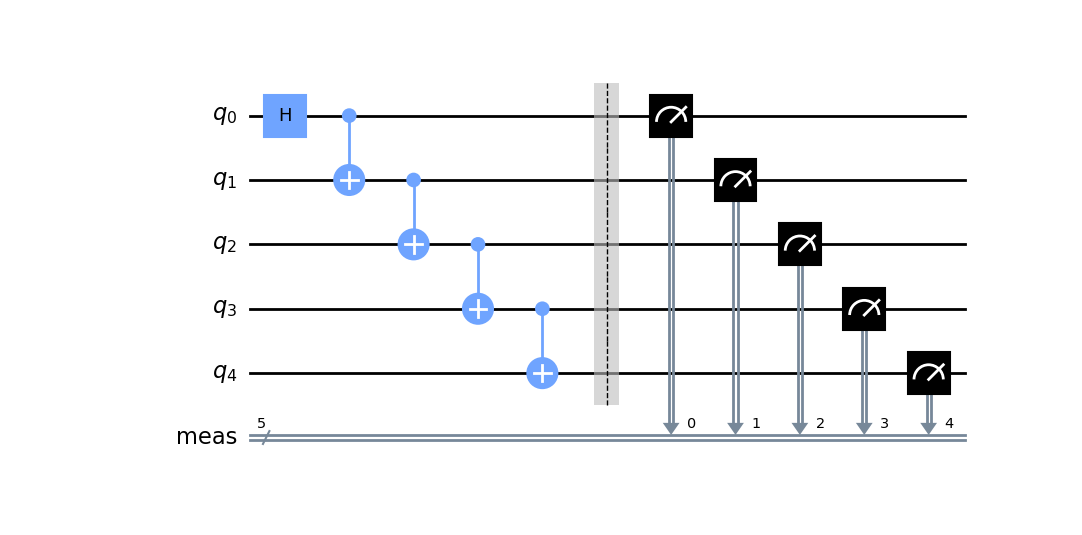
\includegraphics[width=0.75\linewidth]{outputs/ghz.png}
    \caption{GHZ Circuit with $5$ qubits}
    \label{fig:ghz}
\end{figure}
\begin{figure}[hbtp]
    \begin{subfigure}{0.5\linewidth}
        \centering
        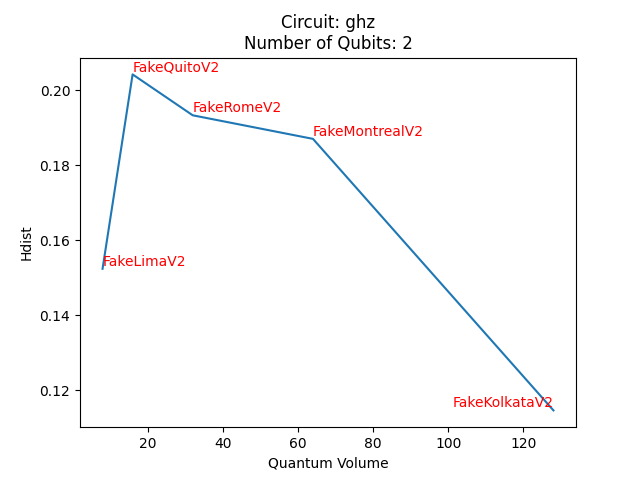
\includegraphics[width=0.9\linewidth]{outputs/ghz_2.png}
    \end{subfigure}
    \begin{subfigure}{0.5\linewidth}
        \centering
        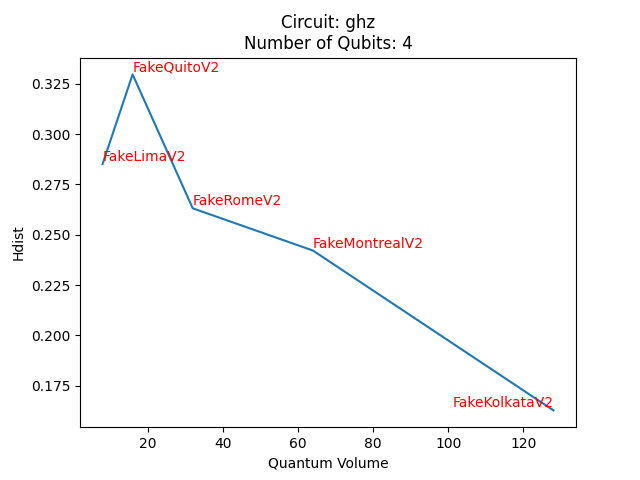
\includegraphics[width=0.9\linewidth]{outputs/ghz_4.png}
    \end{subfigure}
    \begin{subfigure}{\linewidth}
        \centering
        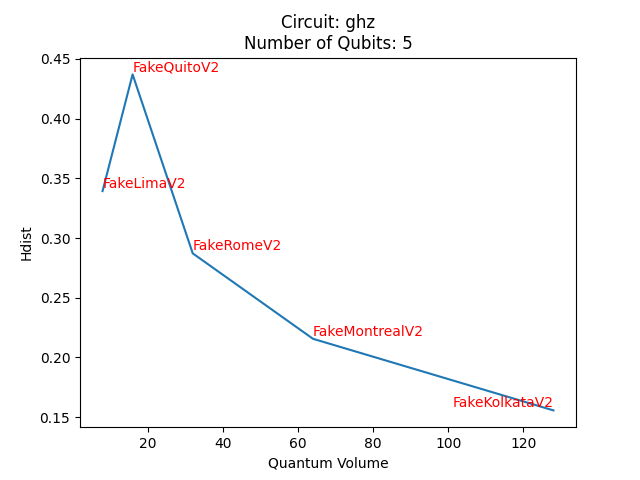
\includegraphics[width=0.45\linewidth]{outputs/ghz_5.png}
    \end{subfigure}
    \caption{Plots of Hellinger distance between statevector simulation and different Quantum Volumes}
    \label{fig:ghzplots}
\end{figure}

As clearly visible from the plots, the natural trend is that the Hellinger distance decreases with increasing Quantum Volume and increases with increasing the number of qubits. This is because the larger the Quantum Volume, the better is the quality of the result on the machine. Similarly, as the number of qubits and gates in the circuit increase, the total error of the circuit increases and hence the Hellinger distance is larger when the circuit has more qubits. However, \texttt{FakeQuitoV2} is an outlier for all the plots. This can easily be inferred from the error map of the machine (Figure~\ref{fig:backends_errormap}) which has a much higher error rate than \texttt{FakeLimaV2} and the other machines.
\begin{figure}[hbtp]
    \begin{subfigure}{0.5\linewidth}
        \centering
        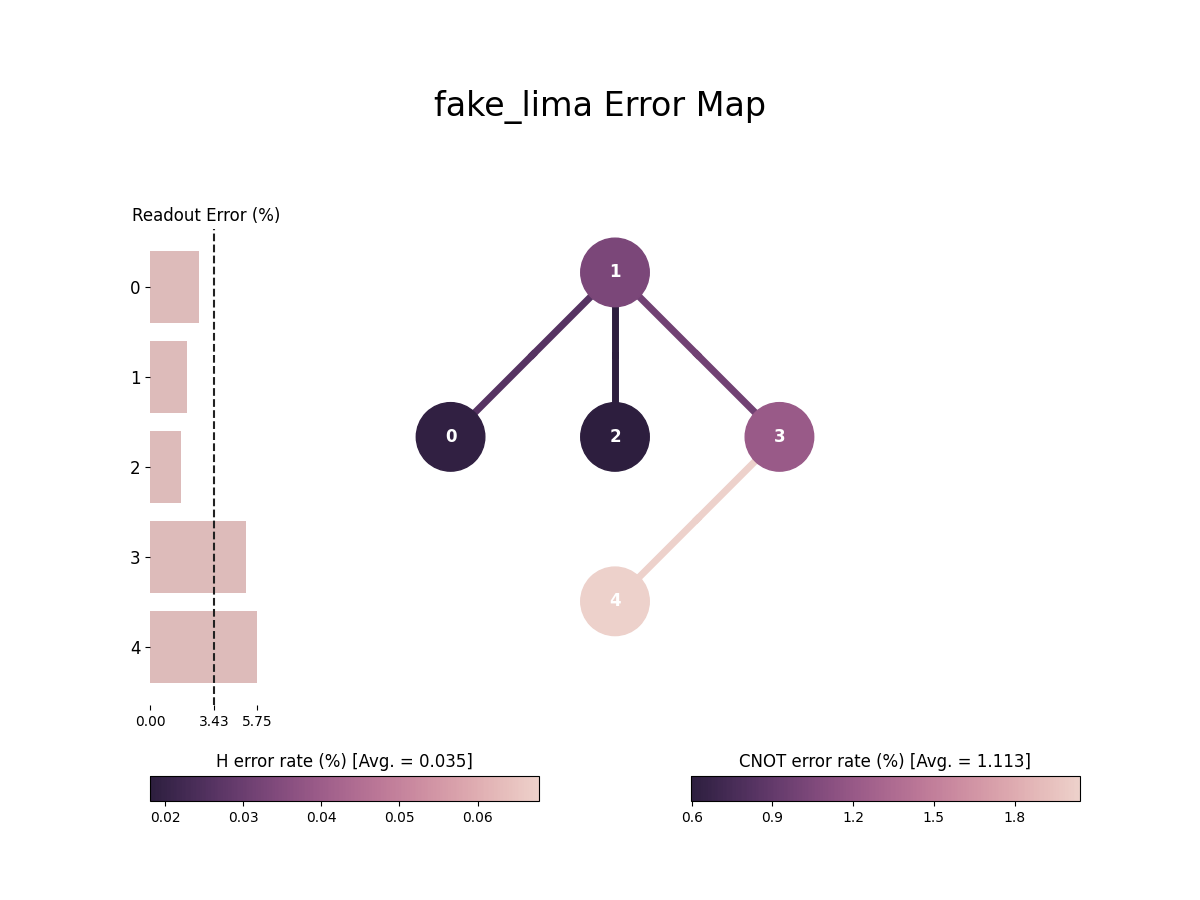
\includegraphics[width=0.9\linewidth]{outputs/errormap_FakeLimaV2.png}
    \end{subfigure}
    \begin{subfigure}{0.5\linewidth}
        \centering
        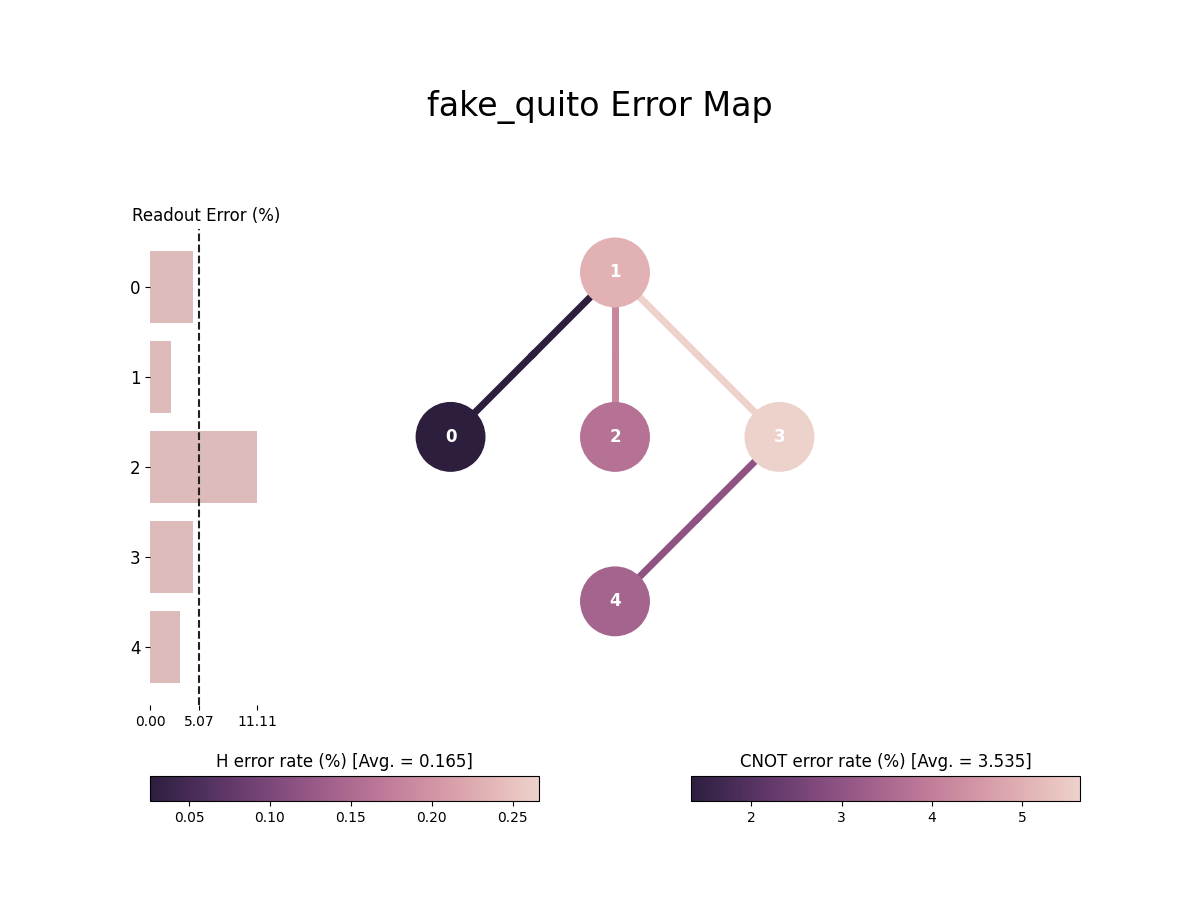
\includegraphics[width=0.9\linewidth]{outputs/errormap_FakeQuitoV2.png}
    \end{subfigure}
    \begin{subfigure}{0.5\linewidth}
        \centering
        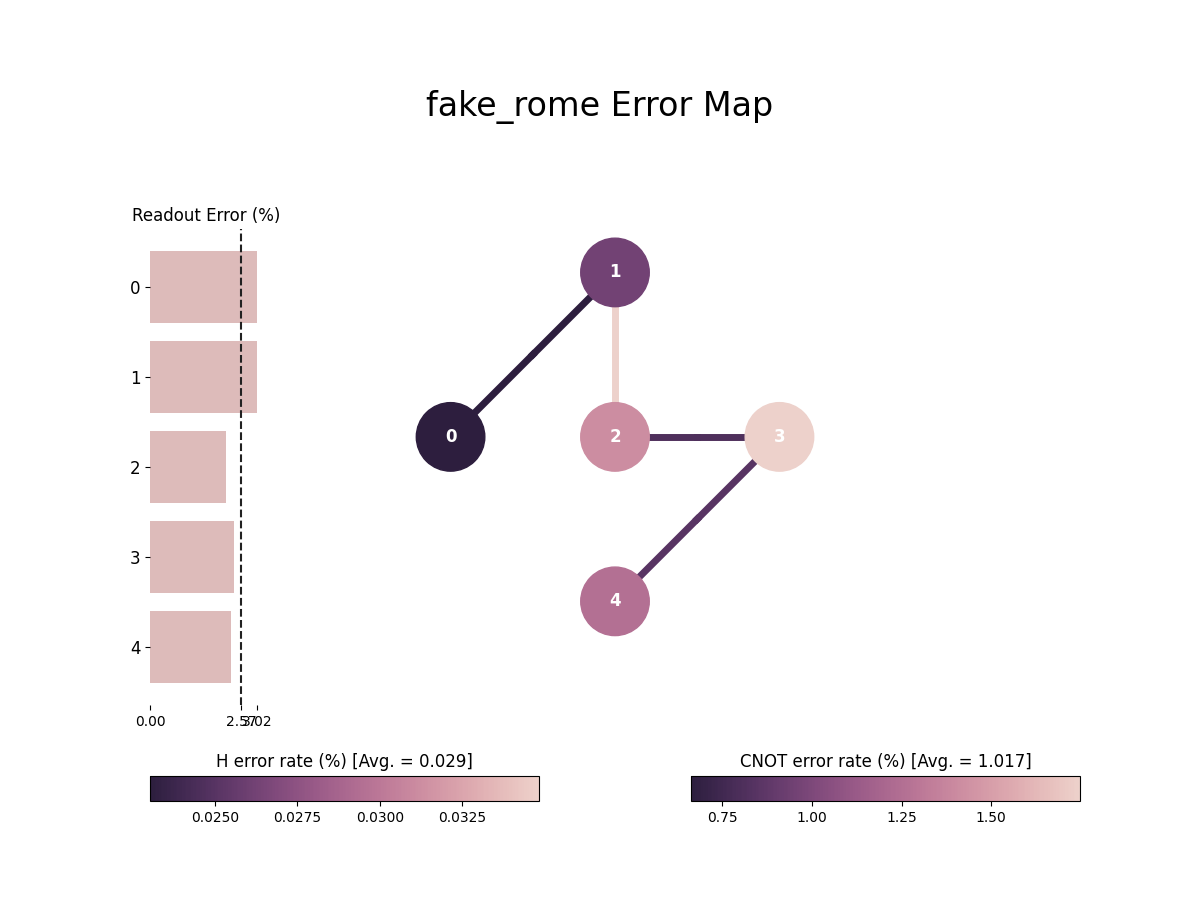
\includegraphics[width=0.9\linewidth]{outputs/errormap_FakeRomeV2.png}
    \end{subfigure}
    \begin{subfigure}{0.5\linewidth}
        \centering
        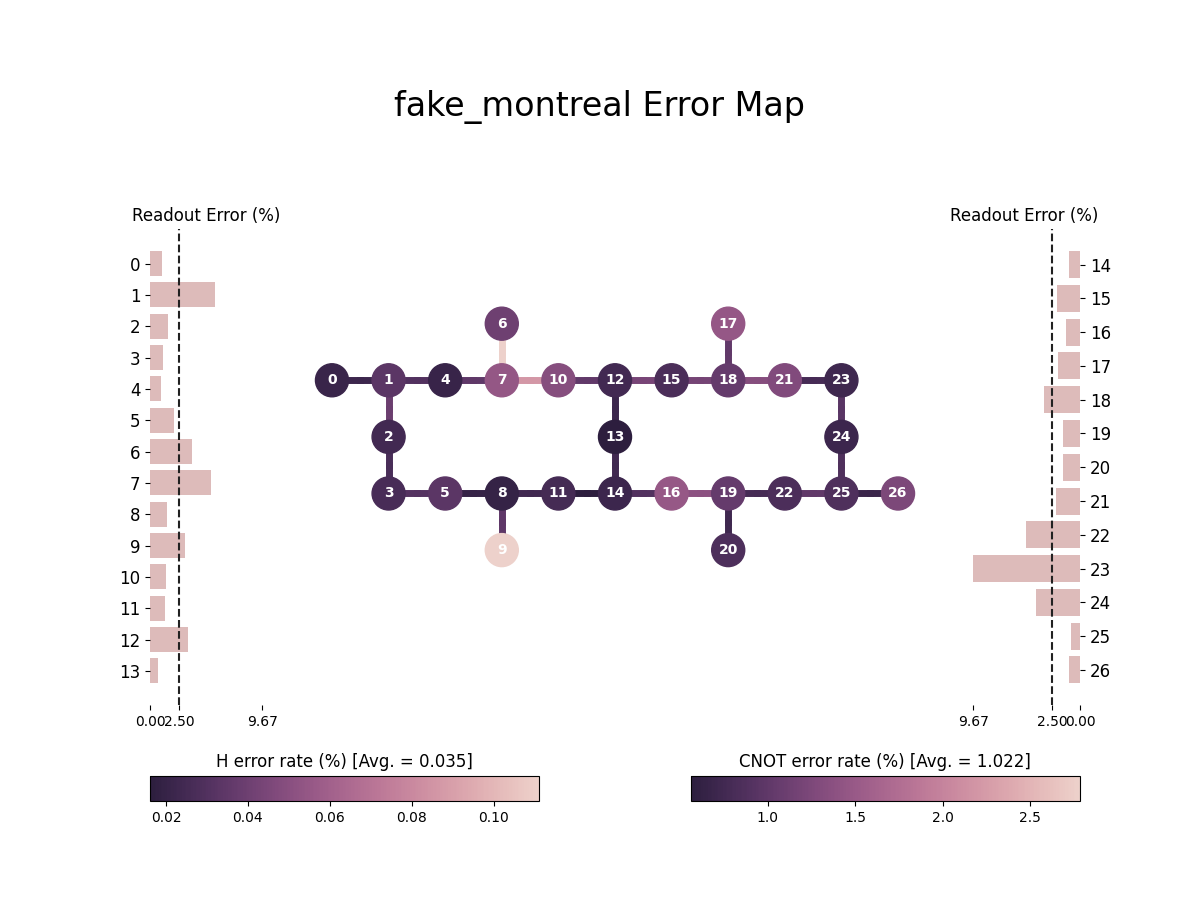
\includegraphics[width=0.9\linewidth]{outputs/errormap_FakeMontrealV2.png}
    \end{subfigure}
    \begin{subfigure}{\linewidth}
        \centering
        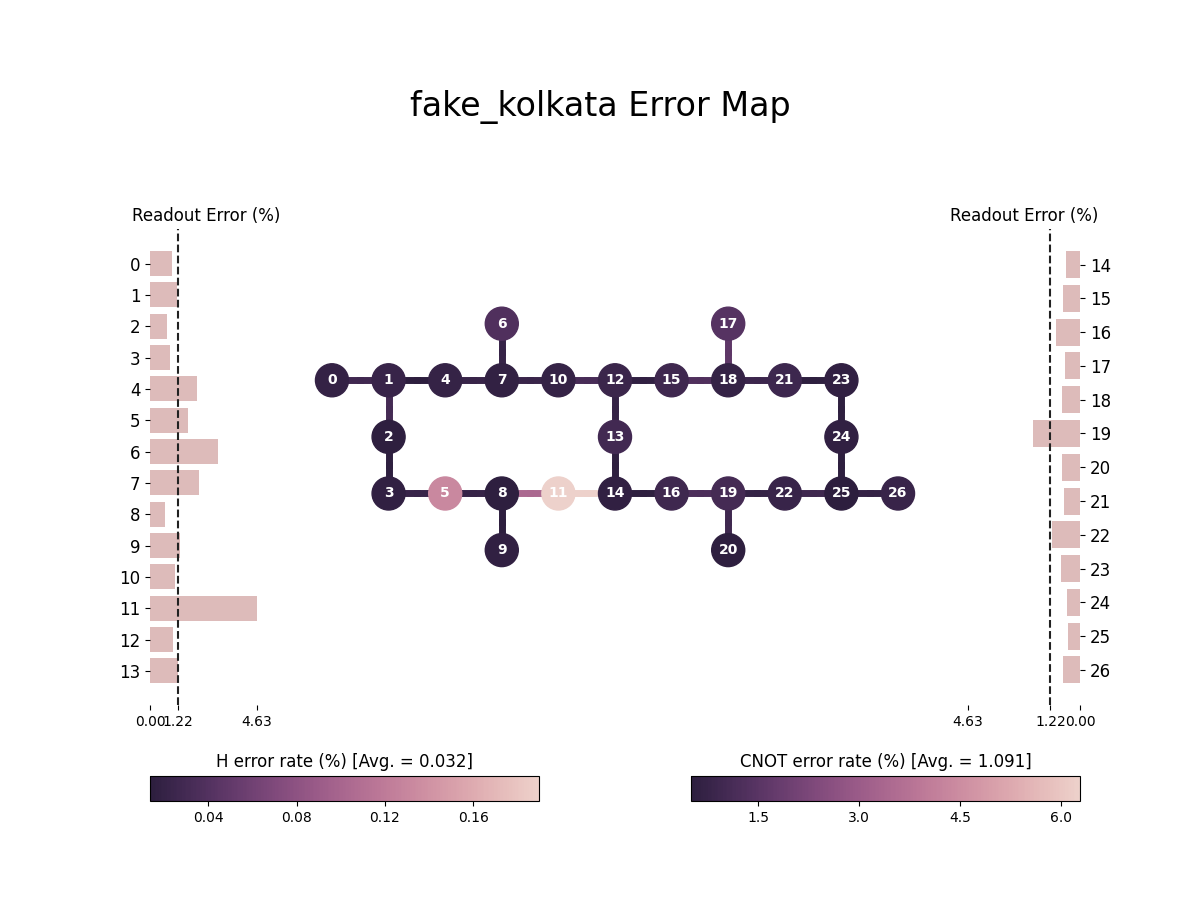
\includegraphics[width=0.45\linewidth]{outputs/errormap_FakeKolkataV2.png}
    \end{subfigure}
    \caption{Error maps of the different backends}
    \label{fig:backends_errormap}
\end{figure}


\subsection{Bernstein-Vazirani Circuit}
An example circuit used for modelling the performance of the Bernstein-Vazirani circuit is shown in Figure~\ref{fig:bv}. The plots for the Bernstein-Vazirani circuit are shown in Figure~\ref{fig:bvplots}.
\begin{figure}[hbtp]
    \centering
    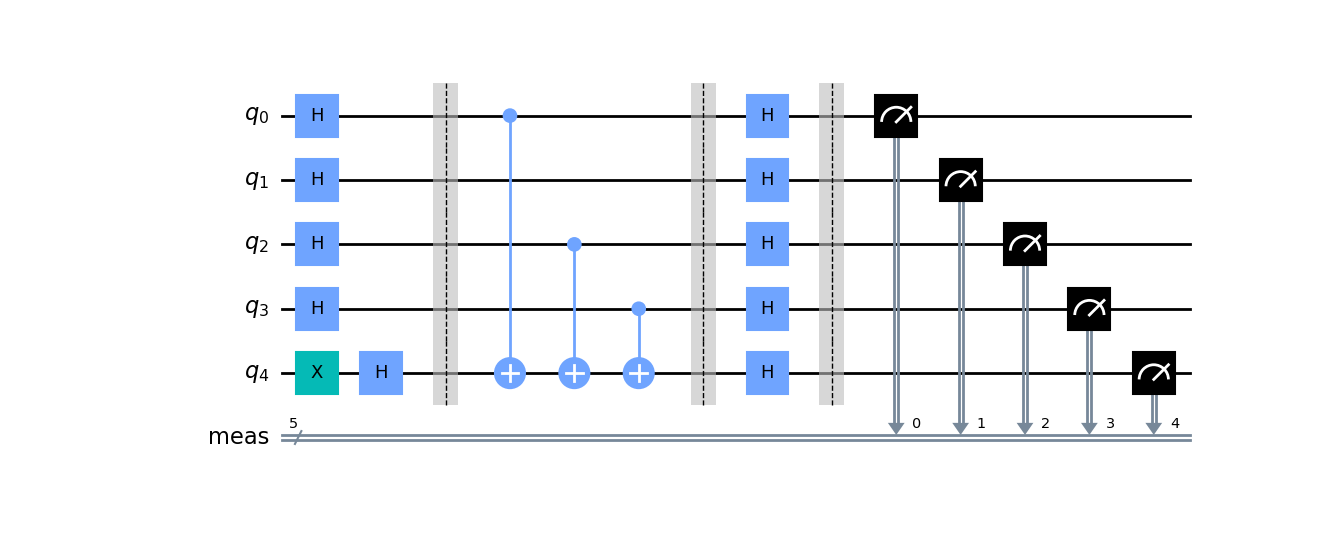
\includegraphics[width=0.75\linewidth]{outputs/bv.png}
    \caption{Bernstein-Vazirani Circuit with $4$ qubits and an ancilla qubit (secret used in $1011$)}
    \label{fig:bv}
\end{figure}
\begin{figure}[hbtp]
    \begin{subfigure}{0.5\linewidth}
        \centering
        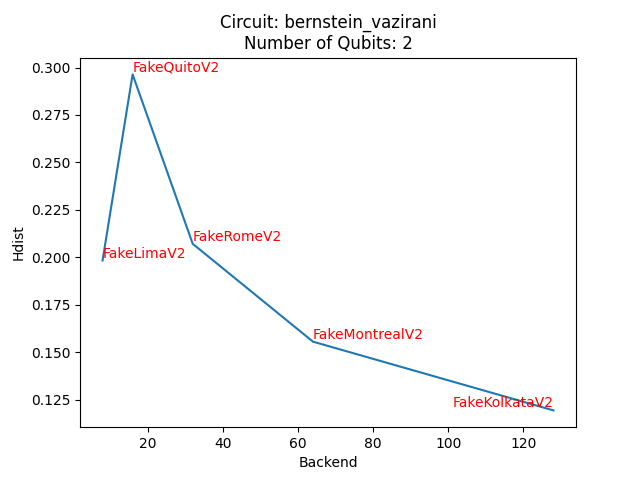
\includegraphics[width=0.9\linewidth]{outputs/bernstein_vazirani_2.png}
        \caption{Secret = $11$}
    \end{subfigure}
    \begin{subfigure}{0.5\linewidth}
        \centering
        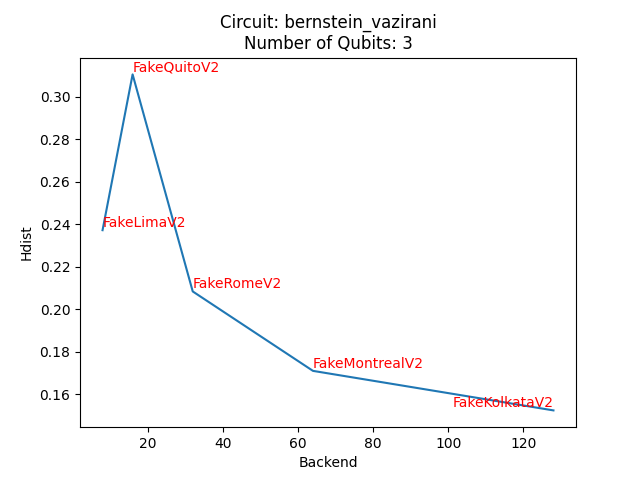
\includegraphics[width=0.9\linewidth]{outputs/bernstein_vazirani_3.png}
        \caption{Secret = $110$}
    \end{subfigure}
    \begin{subfigure}{\linewidth}
        \centering
        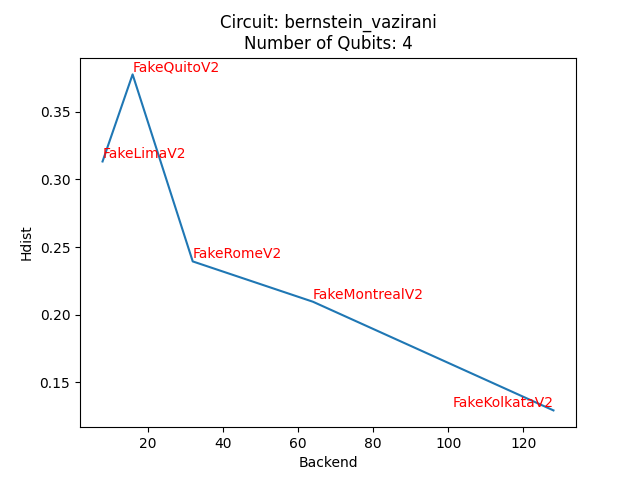
\includegraphics[width=0.45\linewidth]{outputs/bernstein_vazirani_4.png}
        \caption{Secret = $0001$}
    \end{subfigure}
    \caption{Plots of Hellinger distance between statevector simulation and different Quantum Volumes}
    \label{fig:bvplots}
\end{figure}

The trend observed is quite similar to the trends observed in the GHZ circuit. The reason for \texttt{FakeQuitoV2} having a higher error rate than is the same as explained in Section~\ref{ghz}. Otherwise, the Hellinger distance decreases as the Quantum Volume increases which is what we expect. However, the trend for increasing the number of qubits is not so apparent. This is because the circuit complexity does not increase with the increase in the number of qubits. The circuit with $4$ qubits has a much simpler bit-string as the secret due to which the total error does not increase as much in comparison to the circuit for $3$ qubits. In fact, the Hellinger distance for the $4$ qubit circuit is lower than the $3$ qubit circuit for \texttt{FakeKolkataV2}. This is because $5$ qubits is $2$ lower than $\log 128$, which is the maximum number of qubits that were used to get the heavy strings when determining the Quantum Volume of \texttt{FakeKolkataV2}. Therefore, the error is lower when lesser number of gates are used on \texttt{FakeKolkataV2}. This is not the case for the other circuits since the number of qubits used is close to the number of qubits used to compute the Quantum Volume and hence the errors grow considerably.


\section{Grover's Amplitude Amplification}
For this circuit, the metric used is the Hellinger distance between the distribution with a $1$ for the solution bit-string in the database and the distribution obtained from running the circuit on the machine (either statevector or \texttt{FakeKolkataV2}). Again, the circuit was executed for $1024$ shots. The optimal number of iterations for $5$ qubits would be,
\begin{equation}
        \left\lfloor \frac{\pi}{4}\sqrt{\frac{N}{M}} - \frac{1}{2} \right\rfloor = \left\lfloor \frac{\pi}{4}\sqrt{\frac{2^5}{1}} - \frac{1}{2} \right\rfloor = 4
\end{equation}

The Oracle is defined as $\mathbf{I}$ (where $\mathbf{I}$ is the identity matrix) but a $-1$ in the position corresponding to the solution bit-string. The diffuser is defined as $-\mathbf{I}$ but a $1$ for the first row and column.

A sample circuit for solving the Grover's problem is shown in Figure~\ref{fig:grover}. The plots for the Grover's circuit are shown in Figure~\ref{fig:groverplots}.
\begin{figure}[hbtp]
    \centering
    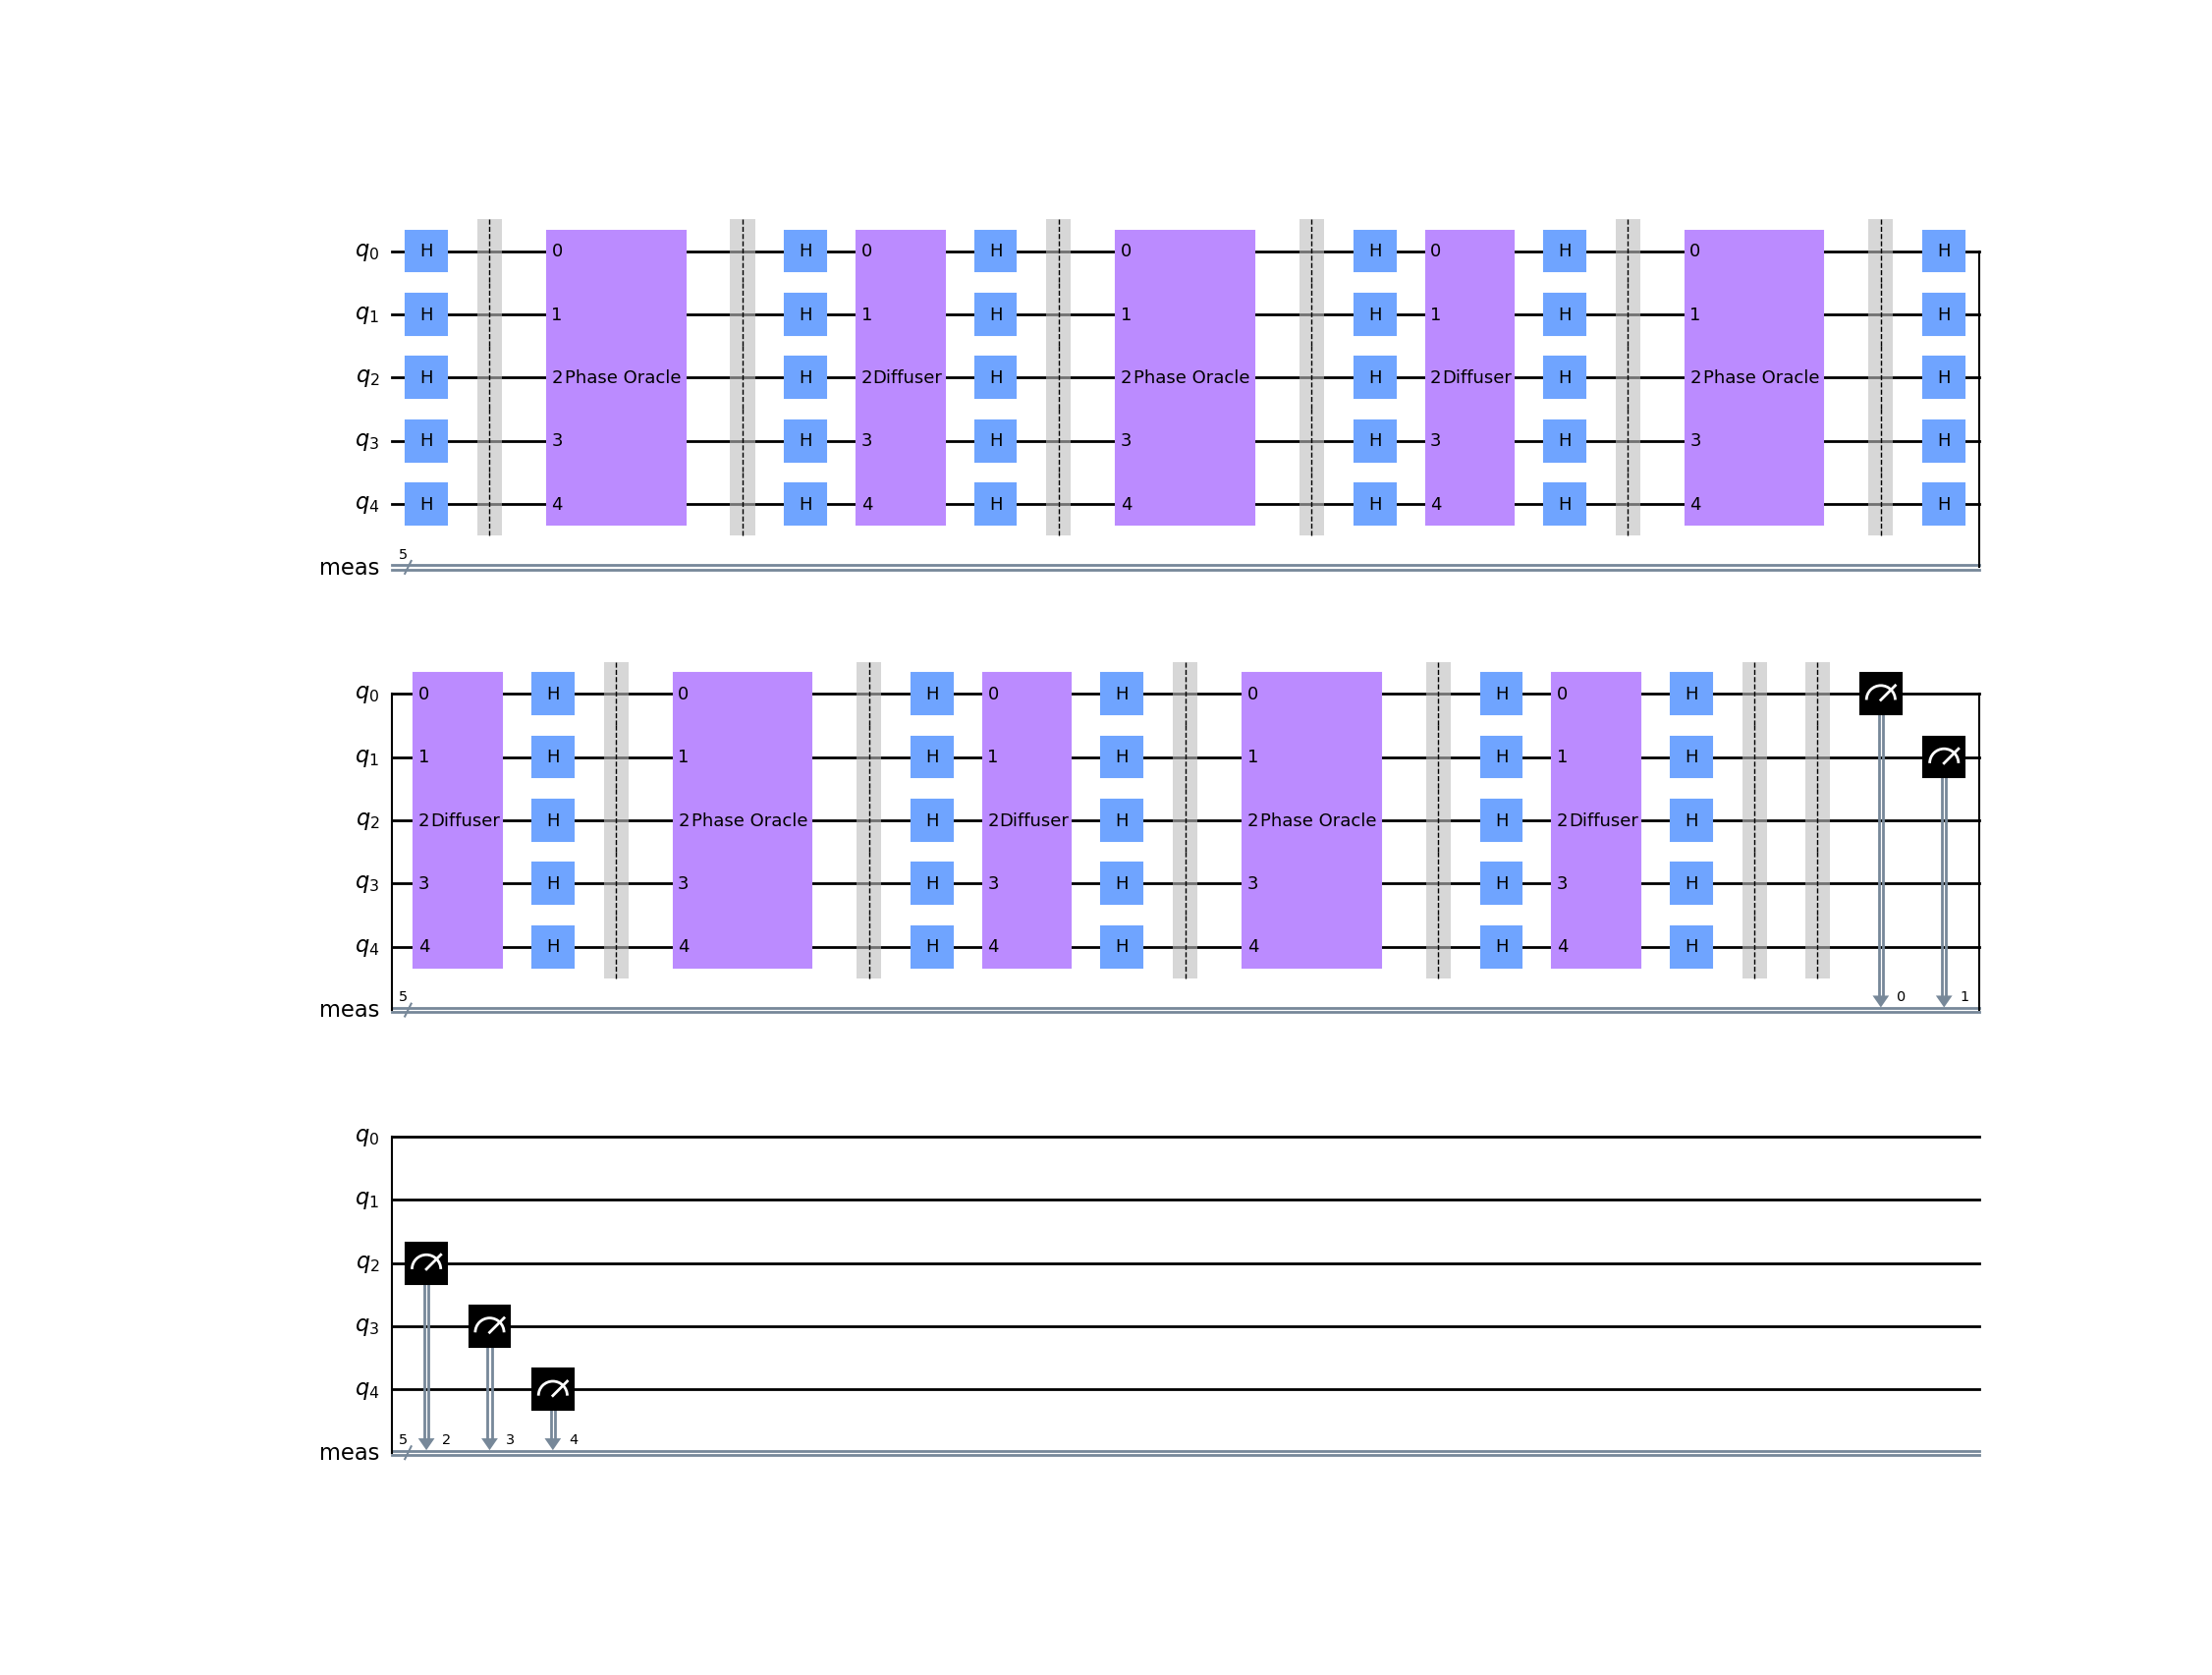
\includegraphics[width=0.8\linewidth]{outputs/grover.png}
    \caption{Grover's Circuit with $5$ qubits and $5$ iterations}
    \label{fig:grover}
\end{figure}
\begin{figure}[hbtp]
    \begin{subfigure}{0.5\linewidth}
        \centering
        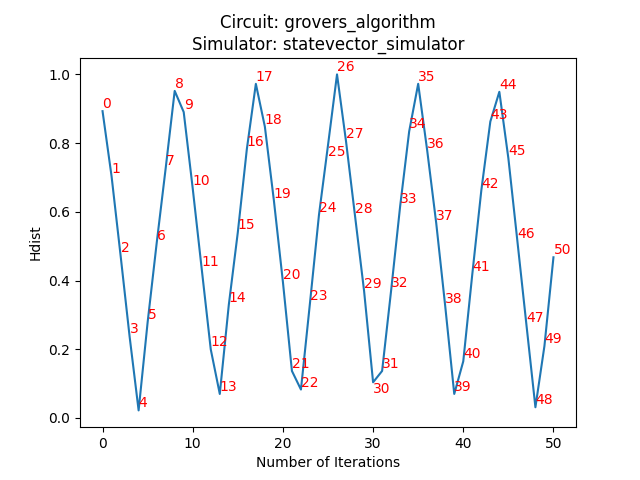
\includegraphics[width=\linewidth]{outputs/grovers_algorithm_statevector_simulator.png}
    \end{subfigure}
    \begin{subfigure}{0.5\linewidth}
        \centering
        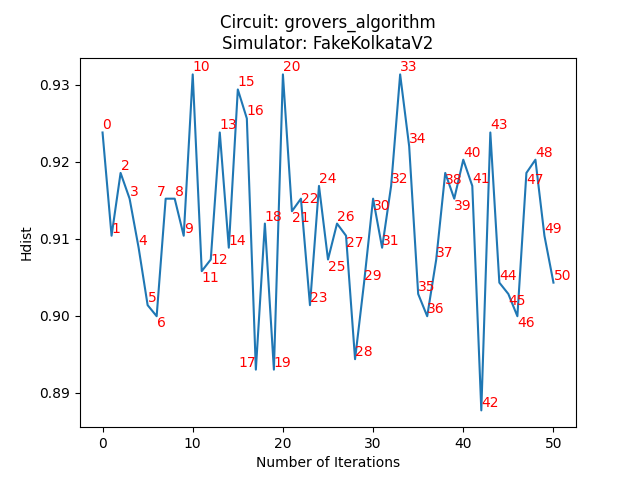
\includegraphics[width=\linewidth]{outputs/grovers_algorithm_FakeKolkataV2.png}
    \end{subfigure}
    \caption{Plots of Hellinger distance for statevector and \texttt{FakeKolkataV2}}
    \label{fig:groverplots}
\end{figure}

The results for the statevector simulation are exactly what they would be theoretically, and we get a Hellinger distance of exactly $0$ for $4$ iterations which verifies our computation. However, for the noisy case, we never get a good result and the output is very noisy for all the iterations. This is because the oracle and diffuser is a $5$-qubit gate which is decomposed into multiple $2$-qubit gates and this greatly increases the error rate of the circuit. The lowest Hellinger distance that we get is for $42$ iterations which is still very large and close to $0.89$ (which is essentially just noise).


\section{Routing}
The error maps for the three architectures considered are shown in Figure~\ref{fig:routing_errormap}. The error map also gives us an idea of the connectivity of the different architectures.
\begin{figure}[hbtp]
    \begin{subfigure}{0.5\linewidth}
        \centering
        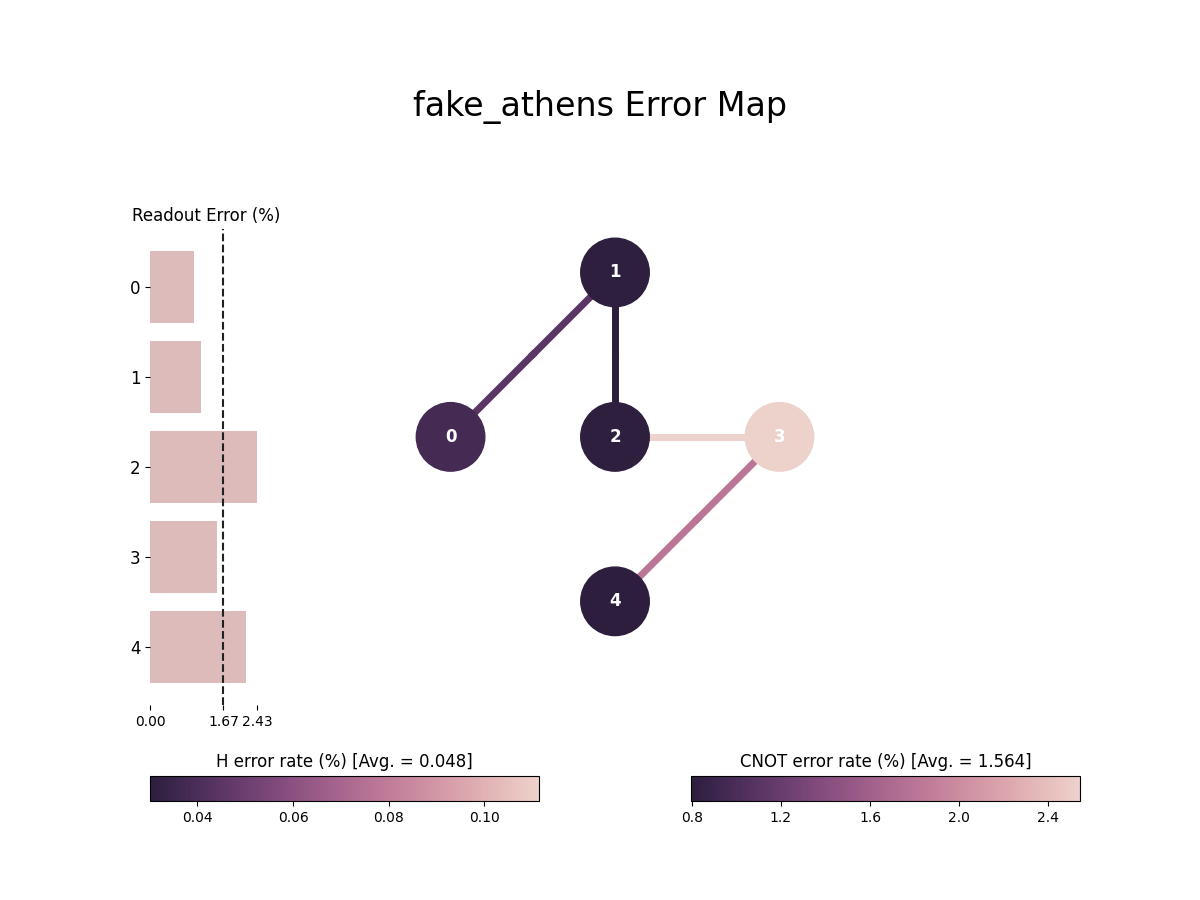
\includegraphics[width=\linewidth]{outputs/errormap_FakeAthensV2.png}
    \end{subfigure}
    \begin{subfigure}{0.5\linewidth}
        \centering
        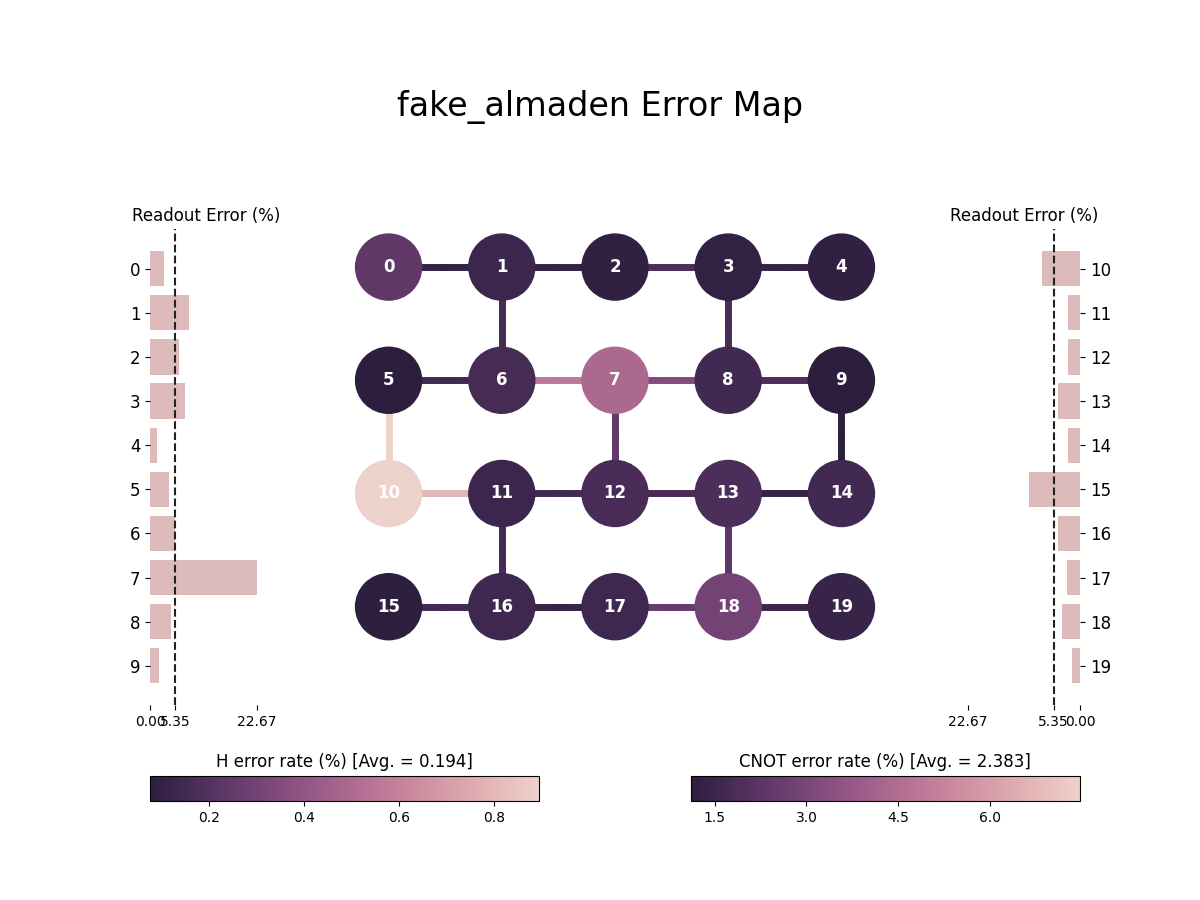
\includegraphics[width=\linewidth]{outputs/errormap_FakeAlmadenV2.png}
    \end{subfigure}
    \begin{subfigure}{\linewidth}
        \centering
        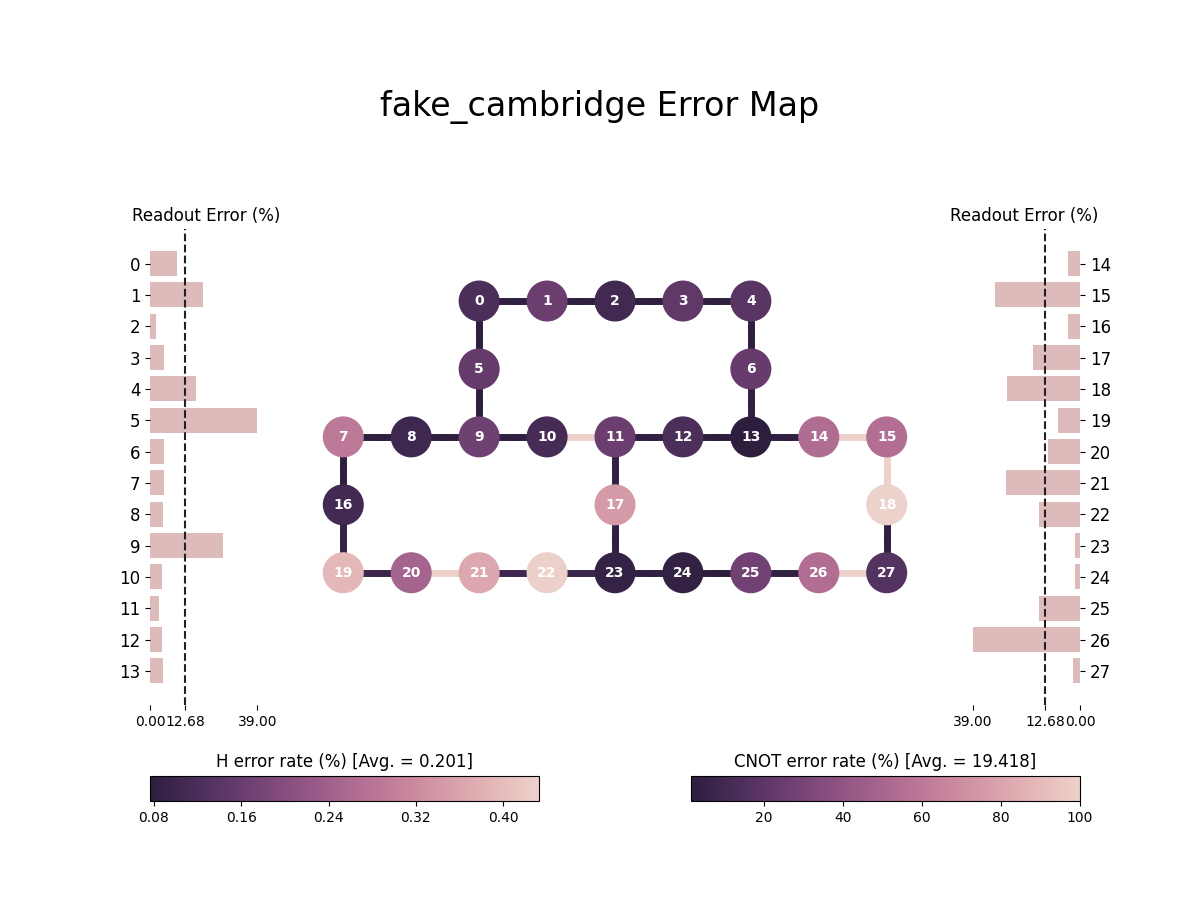
\includegraphics[width=0.66\linewidth]{outputs/errormap_FakeCambridgeV2.png}
    \end{subfigure}
    \caption{Error maps for different architectures}
    \label{fig:routing_errormap}
\end{figure}

\subsection{Routing and Swaps}
The plots for the number of swaps required to execute the \texttt{ComplexCircuit} on the different architectures are shown in Figure~\ref{fig:routing}.
\begin{figure}[hbtp]
    \begin{subfigure}{\linewidth}
        \centering
        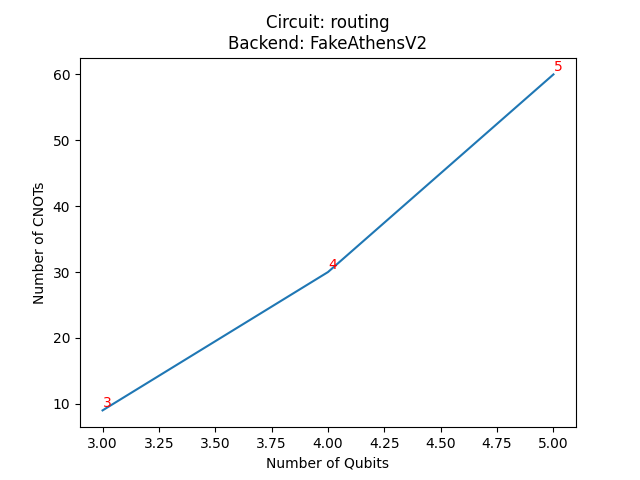
\includegraphics[width=0.5\linewidth]{outputs/routing_FakeAthensV2.png}
    \end{subfigure}
    \begin{subfigure}{0.5\linewidth}
        \centering
        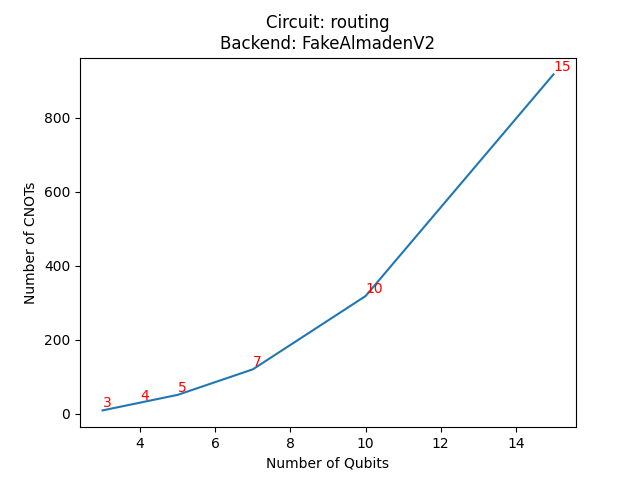
\includegraphics[width=\linewidth]{outputs/routing_FakeAlmadenV2.png}
    \end{subfigure}
    \begin{subfigure}{0.5\linewidth}
        \centering
        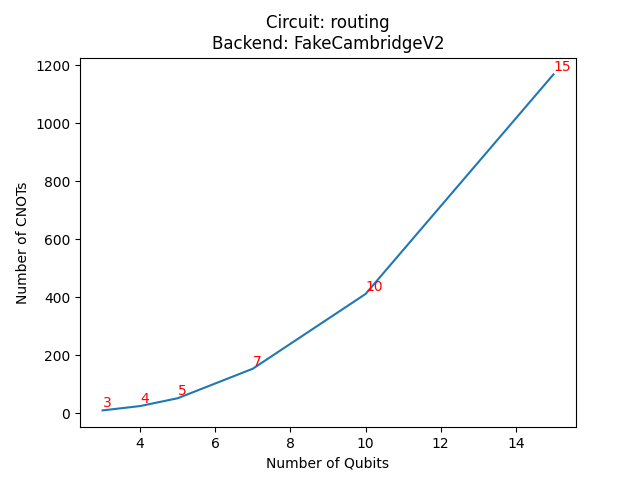
\includegraphics[width=\linewidth]{outputs/routing_FakeCambridgeV2.png}
    \end{subfigure}
    \caption{Number of swaps required for \texttt{ComplexCircuit} on different architectures}
    \label{fig:routing}
\end{figure}

The number of swaps required for \texttt{FakeAlmadenV2} is the least since its architecture has the maximum connectivity. On the contrary, \texttt{FakeCambridgeV2} has the highest number of swaps required since there is limited connectivity among the qubits even though it has more qubits. The number of swaps required for \texttt{FakeAthensV2} is almost the same as \texttt{FakeCambridgeV2} since the connectivity for the first $5$ qubits is the same for both the architectures. The number of swaps required for \texttt{FakeCambridgeV2} is slightly lesser since it has more qubits to allow for slightly more flexibility, and it doesn't need to always work with just $5$ qubits in total.

\subsection{Noise Adaptive Routing}
For all architectures, the Bernstein-Vazirani circuit was chosen with the secret key $1111$ to introduce the maximum number of \texttt{CNOTs} and hence be able to easily differentiate between the algorithms used at different optimization levels.
\subsubsection{\texttt{FakeAthensV2}}
The mappings for different optimization options are shown Figure~\ref{fig:routing_athens}. Data qubit $4$ is the only qubit that has CNOTs with all other qubits and hence it should be placed in a position with low \texttt{CNOT} error rates. Therefore, in \texttt{optimization\_level} $1$ data qubit $4$ is placed in physical qubit $1$ of the architecture. However, \texttt{optimization\_level} $2$ and $3$ instead place data qubit $4$ in the position of logical qubit $2$ since this leads to reduced number of \texttt{SWAP} insertions even though it increases the actual \texttt{CNOT} error rate for a few gates in the original circuit, thus reducing the combined error rate of the circuit.
\begin{figure}[hbtp]
    \begin{subfigure}{0.24\linewidth}
        \centering
        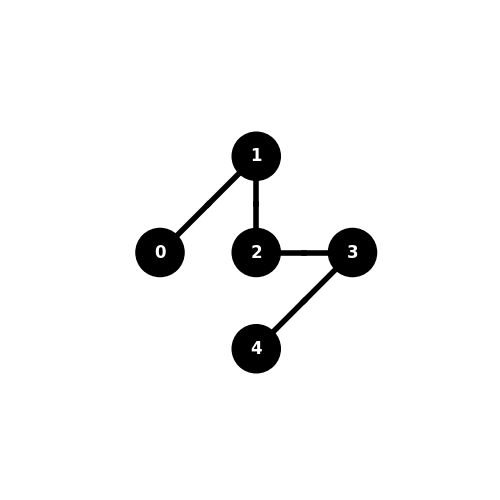
\includegraphics[width=\linewidth]{outputs/routing_FakeAthensV2_0.png}
        \caption{\texttt{optimization\_level} $0$}
    \end{subfigure}
    \begin{subfigure}{0.24\linewidth}
        \centering
        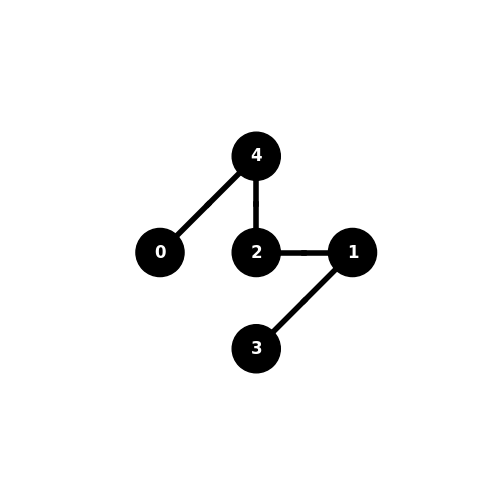
\includegraphics[width=\linewidth]{outputs/routing_FakeAthensV2_1.png}
        \caption{\texttt{optimization\_level} $1$}
    \end{subfigure}
    \begin{subfigure}{0.24\linewidth}
        \centering
        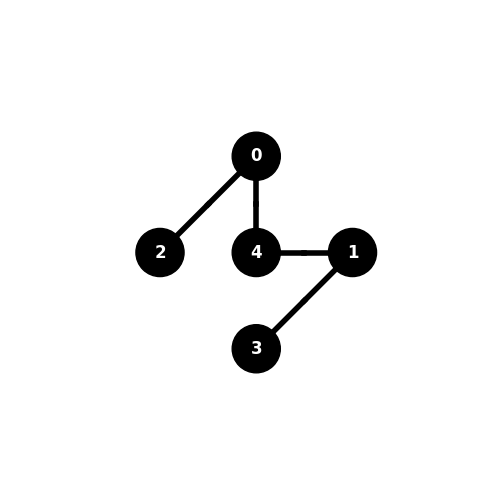
\includegraphics[width=\linewidth]{outputs/routing_FakeAthensV2_2.png}
        \caption{\texttt{optimization\_level} $2$}
    \end{subfigure}
    \begin{subfigure}{0.24\linewidth}
        \centering
        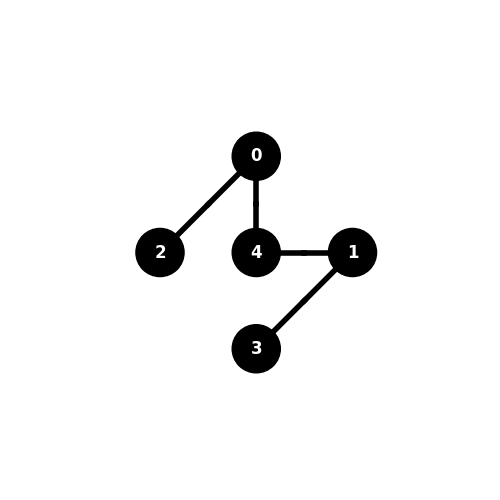
\includegraphics[width=\linewidth]{outputs/routing_FakeAthensV2_3.png}
        \caption{\texttt{optimization\_level} $3$}
    \end{subfigure}
    \caption{Mappings for different optimization levels for \texttt{FakeAthensV2}}
    \label{fig:routing_athens}
\end{figure}

\subsubsection{\texttt{FakeAlmadenV2}}
The mappings for different optimization options are shown Figure~\ref{fig:routing_almaden}. All the (non-zero) optimization levels try to place the data qubits so that there is maximum connectivity between data qubit $4$ and the other qubits while also ensuring that the \texttt{CNOT} error rates are low. Similar to the previous part, \texttt{optimization\_level} $1$ optimizes for reduced \texttt{CNOT} error rates. \texttt{optimization\_level} $2$ optimizes for reduced number of swaps and \texttt{optimization\_level} $3$ balances between the two.
\begin{figure}[hbtp]
    \begin{subfigure}{0.24\linewidth}
        \centering
        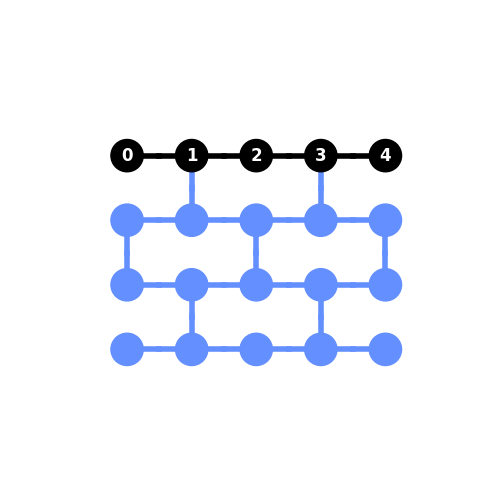
\includegraphics[width=\linewidth]{outputs/routing_FakeAlmadenV2_0.png}
        \caption{\texttt{optimization\_level} $0$}
    \end{subfigure}
    \begin{subfigure}{0.24\linewidth}
        \centering
        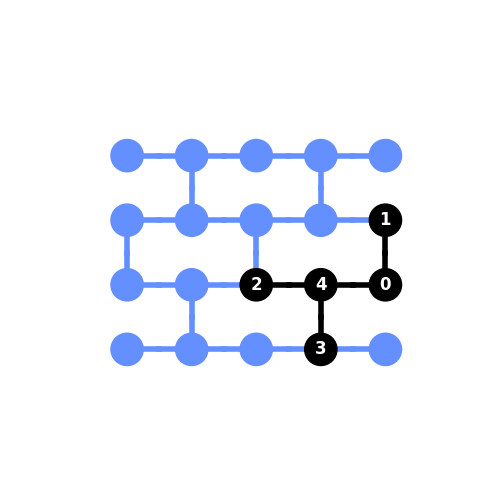
\includegraphics[width=\linewidth]{outputs/routing_FakeAlmadenV2_1.png}
        \caption{\texttt{optimization\_level} $1$}
    \end{subfigure}
    \begin{subfigure}{0.24\linewidth}
        \centering
        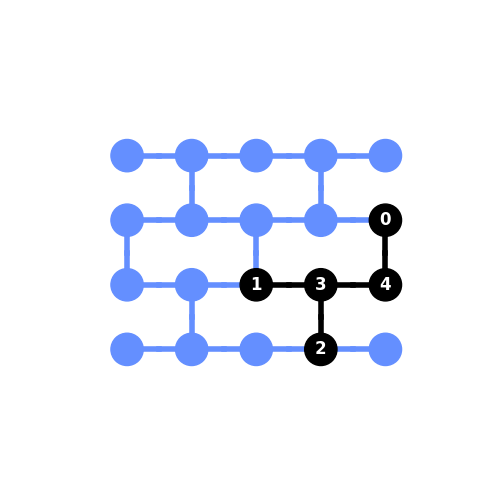
\includegraphics[width=\linewidth]{outputs/routing_FakeAlmadenV2_2.png}
        \caption{\texttt{optimization\_level} $2$}
    \end{subfigure}
    \begin{subfigure}{0.24\linewidth}
        \centering
        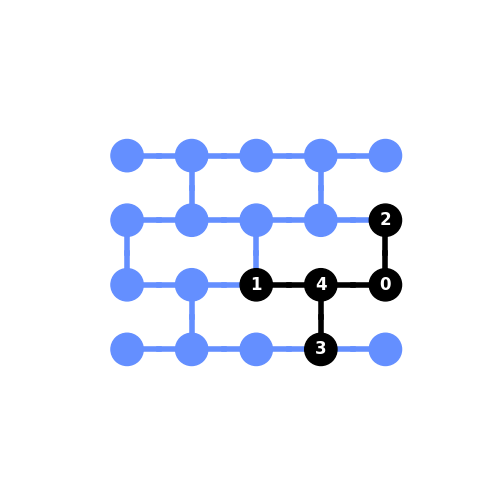
\includegraphics[width=\linewidth]{outputs/routing_FakeAlmadenV2_3.png}
        \caption{\texttt{optimization\_level} $3$}
    \end{subfigure}
    \caption{Mappings for different optimization levels for \texttt{FakeAlmadenV2}}
    \label{fig:routing_almaden}
\end{figure}

\subsubsection{\texttt{FakeCambridgeV2}}
The mappings for different optimization options are shown Figure~\ref{fig:routing_cambridge}. The placement is chosen so that the two-qubit gates have the least errors and the minimal number of swaps are introduced. \texttt{optimization\_level} $1$ chooses the arrangement that minimizes the individual \texttt{CNOT} error rates. \texttt{optimization\_level} $2$ chooses the placement that minimizes the number of swaps and hence leads to a hole between the qubits since whichever qubit has to perform a \texttt{CNOT} with the data qubit $4$ can swap with the empty qubit which would require one lesser \texttt{CNOT} gate. Finally, \texttt{optimization\_level} $3$ balances between the two and hence places data qubit $4$ in the most accessible position and in the middle of the other qubits.
\begin{figure}[hbtp]
    \begin{subfigure}{0.24\linewidth}
        \centering
        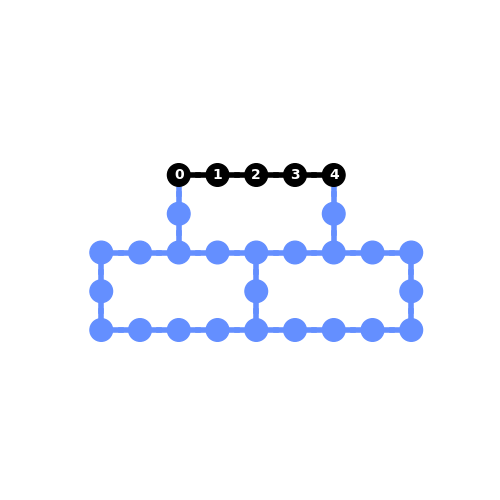
\includegraphics[width=\linewidth]{outputs/routing_FakeCambridgeV2_0.png}
        \caption{\texttt{optimization\_level} $0$}
    \end{subfigure}
    \begin{subfigure}{0.24\linewidth}
        \centering
        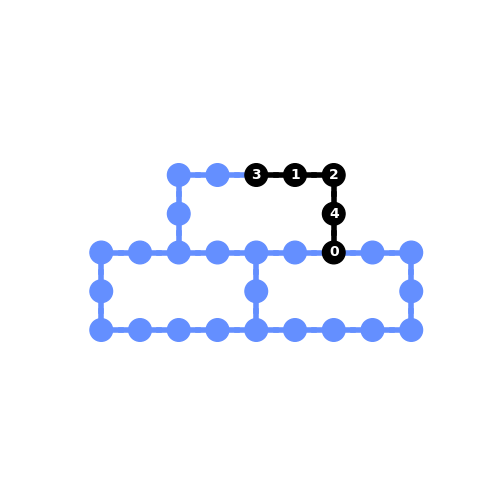
\includegraphics[width=\linewidth]{outputs/routing_FakeCambridgeV2_1.png}
        \caption{\texttt{optimization\_level} $1$}
    \end{subfigure}
    \begin{subfigure}{0.24\linewidth}
        \centering
        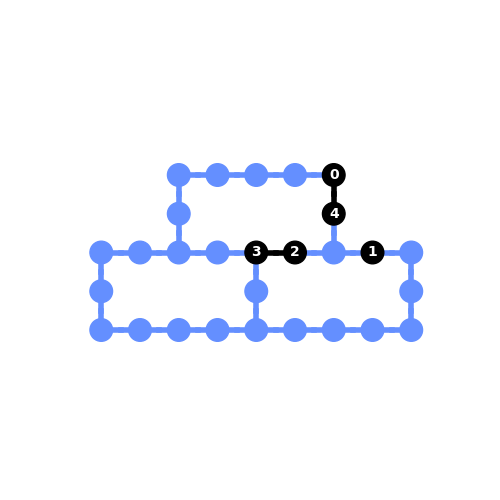
\includegraphics[width=\linewidth]{outputs/routing_FakeCambridgeV2_2.png}
        \caption{\texttt{optimization\_level} $2$}
    \end{subfigure}
    \begin{subfigure}{0.24\linewidth}
        \centering
        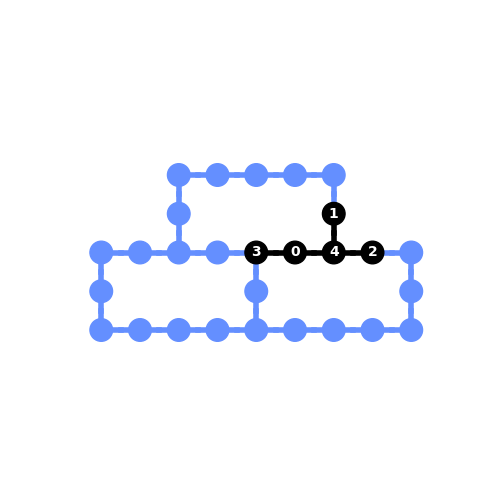
\includegraphics[width=\linewidth]{outputs/routing_FakeCambridgeV2_3.png}
        \caption{\texttt{optimization\_level} $3$}
    \end{subfigure}
    \caption{Mappings for different optimization levels for \texttt{FakeCambridgeV2}}
    \label{fig:routing_cambridge}
\end{figure}


\section{Conclusion}
Thus, in the lab we analyzed various Quantum Algorithms and the routing and placement problem for quantum compilers. We observed that the quantum computers at their current state cannot be used even for some of the simple circuits that can be easily computed classically (since the sizes are very small). However, we also observed that the different routing and placement algorithms that take advantage of the device level metrics strive towards reducing the errors and are quite successful in doing so, at least for small devices since the search spaces are small. This also leads us to realize that there is plenty of scope for research in this domain so that there are state-of-the-art compilers by the time we have devices that have enough qubits to actually run circuits with practical advantages.


\end{document}